\documentclass[12pt]{article}

\usepackage{sbc-template}
\usepackage{graphicx,url}
\usepackage[brazil]{babel}   
\usepackage[utf8]{inputenc}  
    
\sloppy

\title{Recuperação de Informação -- Relatório do Trabalho Prático 1}
\author{Danilo Ferreira e Silva\inst{1}}
\address{Departamento de Ciência da Computação -- UFMG
  \email{danilofes@gmail.com}
}

\begin{document} 

\maketitle

\begin{resumo}
  Este relatório descreve o desenvolvimento do trabalho prático 1, proposto na 
  disciplina Recuperação de Informação. O trabalho consistiu da implementação de um
  indexador e processador de consultas simples, aplicando o conhecimento aprendido em
  aula. Experimentos realizados no sistema desenvolvido mostraram que ele é capaz de gerar
  índices, na forma de listas invertidas, para coleções da ordem de 400 mil documentos
  em aproximadamente uma hora.
\end{resumo}


\section{Arquitetura do sistema} \label{sec:firstpage}

O sistema foi construído na linguagem C++, conforme especificado, e é constituido de 
dois executáveis. O primeiro deles é o indexador da coleção de documentos, que gera 
um arquivo de listas invertidas ao final do processamento.
O segundo é o processador de consultas, que usa o arquivo gerado pelo
indexador para responder a consultas do usuário de forma interativa, via linha de
comando.


\subsection{Módulos e dependências}

Na figura~\ref{fig:modules} são apresentados os módulos e dependências entre eles.

\begin{figure}[ht]
\centering
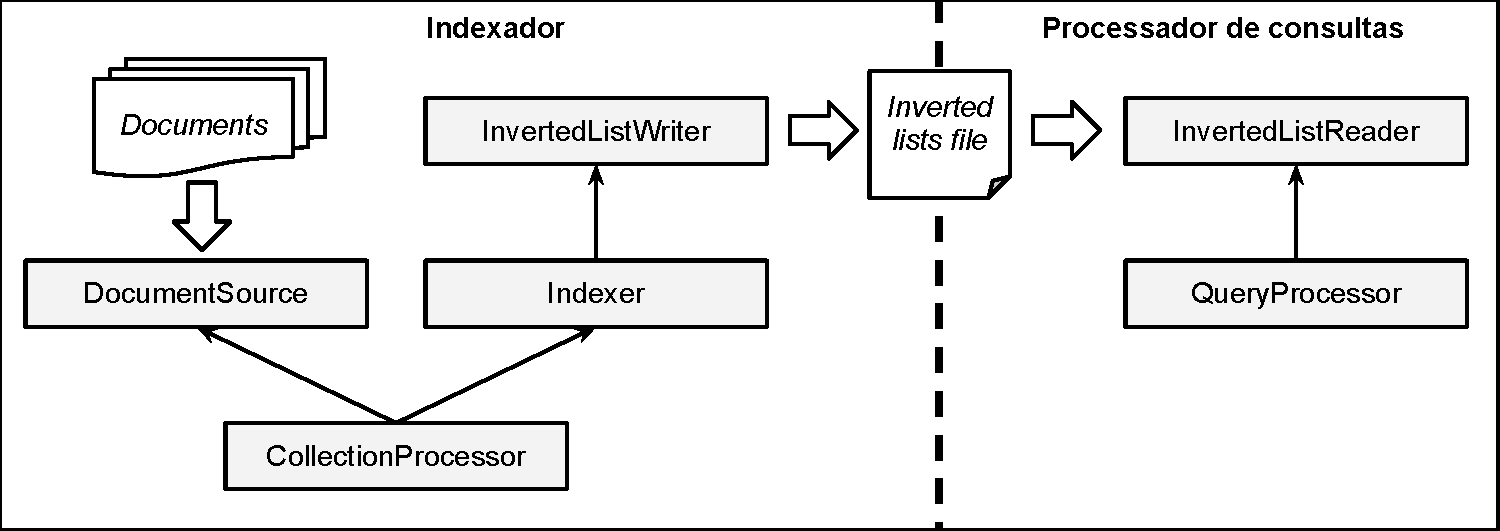
\includegraphics[width=1\textwidth]{modules.pdf}
\caption{Diagrama de dependências de módulos do sistema}
\label{fig:modules}
\end{figure}

\begin{description}
\item[DocumentSource] Abstração que representa uma fonte de documentos, identificados por uma URL e cujo conteúdo é uma sequência de caracteres. A implementação lê os documentos usando a RICPlib.
\item[CollectionProcessor] Módulo principal que lê um conjunto de documentos fornecidos pelo \emph{DocumentSource}, transforma-os em uma sequência de termos e alimenta o \emph{Indexer}.
\item[Indexer] Recebe um conjunto de termos dos documentos e faz a indexação. Ao final escreve as listas invertidas usando o \emph{InvertedListWriter}.
\item[InvertedListWriter] Escreve o arquivo de listas invertidas.
\item[InvertedListReader] Lê o arquivo de listas invertidas.
\item[QueryProcessor] Processa uma consulta e devolve os resultados.
\end{description}


\subsection{Dependência a bibliotecas de terceiros}

O sistema foi contruído usando a API padrão C++11. Além disso, foram utilizadas as bibliotecas listadas a seguir.

\begin{description}
\item[RICPlib] Biblioteca fornecida na especificação para ler a coleção de documentos comprimida.
\item[zlib] Dependência indireta induzida pela RICPlib.
\item[htmlcxx] Parser de documentos HTML.
\item[gmock] Biblioteca para criação de \textit{mock objects} (usada apenas em testes unitários).
\end{description}


\section{Algoritmos e estruturas de dados utilizados}

O processo de indexação pode ser subdividido nas três etapas descritas abaixo:
\begin{enumerate}
\item Leitura dos documentos e escrita das triplas no arquivo temporário.
\item Ordenação das triplas, subdivididas em vários blocos de acordo com o tamanho do buffer.
\item \emph{Merge} dos blocos, e geração das listas invertidas.
\end{enumerate}

Na etapa 1, a principal estrutura de dados envolvida é o vocabulário. Ele é representado internamente por uma tabela \emph{hash}, onde a chave é o próprio termo. Cada entrada da mesma também contém um identificador numérico atribuído ao termo e um contador de ocorrências do termo em documentos. Adicionalmente, ao processar um documento, é criado uma estrutura para guardar o vocabulário local, tembém usando uma tabela \emph{hash}. Nesta a chave é o identificador do termo, e a entrada é um contador de frequência do termo no documento.

Portanto, para cada termo de cada documento, consulta-se primeiro o vocabulário para obter o identificador do termo (ou criar um novo). Em seguida é consultado o vocabulário local, para atualizar a frequência do mesmo no documento. Ambas as operações são $O(1)$, portanto a primeira etapa tem custo de tempo linear com relação ao número total de termos. O custo de memória é proporcional ao número de termos distintos.


\subsection{Ordenação externa das triplas}

As etapas 2 e 3 do algoritmo são na verdade uma ordenação externa. Para que seja viável indexar uma grande coleção de documentos, o índice não pode ser mantido todo em memória. Isso torna necessário o uso da ordenação externa.

A etapa 2 consiste na primeira etapa da ordenação das triplas no arquivo invertido, onde o conjunto de triplas são divididos em blocos menores de tamanho constante $k$. Para cada um desses blocos, é feita uma ordenação em memória usando o algoritmo \emph{heapsort}, cujo custo é $O(n \log{n})$.

Consideranto $T$ o número total de triplas, o custo dessa etapa é aproximadamente: 
$$\lceil T/k \rceil k \log{k}$$
que é linear para efeitos práticos, pois $\log{k}$ é uma constante.

Finalmente na etapa 3, é feita uma intercalação de múltiplos caminhos nos $R = \lceil T/k \rceil$ blocos ordenados em disco. Para isso é utilizado um \emph{heap} de tamanho $R$. Para cada tripla retirada do mesmo, ele é reconstruído com custo logaritmico. O custo total pode ser aproximado como:
$$T \log{\lceil T/k \rceil}$$



\section{Avaliação}

Para avaliar o desempenho do sistema, foram executados experimentos com tamanhos variados de coleções de documento, e também com tamanhos variados de \emph{buffer} usado na ordenação externa.

O indexador é executado pelo binário \emph{indexp}, e pode receber como parâmetros:
\begin{description}
\item[-d inputDirectory] Diretório que contém os arquivos da coleção.
\item[-i indexFileName] Nome do arquivo de índice, que deve estar dentro do mesmo diretório da coleção.
\item[-b bufferSize] Tamanho do buffer (em número de triplas) usado na ordenação externa.
\end{description}

Na figura~\ref{fig:indexp} temos uma saída típica da execução do indexador, mostrando algumas estatísticas básicas coletadas.

O processador de consultas é executado pelo binário \emph{queryp}. No momento ele busca resultados que contém todos os termos, assumindo sempre o operador \emph{and}.


\begin{figure}[ht]
\centering
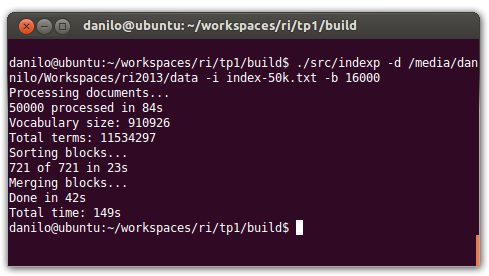
\includegraphics[width=.8\textwidth]{indexp-output.png}
\caption{Execução típica do indexador}
\label{fig:indexp}
\end{figure}

\subsection{Tempo de indexação}\label{sec:time}

A tabela~\ref{tab:exec_time_collection} mostra o tempo de execução total e de cada uma das três etapas para coleções de tamanhos variados e com \emph{buffer} de tamanho 16000. O tempo total de execução cresceu de forma prevista, próxima de linear, até o tamanho de 200000 documentos, conforme o gráfico~\ref{fig:time_vs_colsize}. Para 400000 documentos o tempo aumentou consideravelmente, indicando algum fator extra que influenciou negativamente a performance. Este comportamento foi exclusivo na etapa 3, onde, ao dobrar o número de documentos, o tempo aumentou proximadamente por um fator de $18$. Este fato ainda está sendo investigado e não cheguei a uma explicação definitiva até o momento.


\begin{table}[ht]
\centering
\caption{Tempo de execução em segundos para entradas de tamanho variado}
\label{tab:exec_time_collection}
\begin{tabular}{rrrrr}
Documentos  & Etapa 1 & Etapa 2 & Etapa 3 & Total \\ \hline
5000        & 8      & 1      & 2      & 11 \\
10000       & 15     & 3      & 4      & 22 \\
50000       & 83     & 20     & 26     & 129 \\
100000      & 166    & 51     & 56     & 273 \\
150000      & 263    & 80     & 87     & 430 \\
200000      & 340    & 112    & 149    & 601 \\
400000      & 688    & 230    & 2659   & 3577 \\
\end{tabular}
\end{table}


\begin{figure}[ht]
\centering
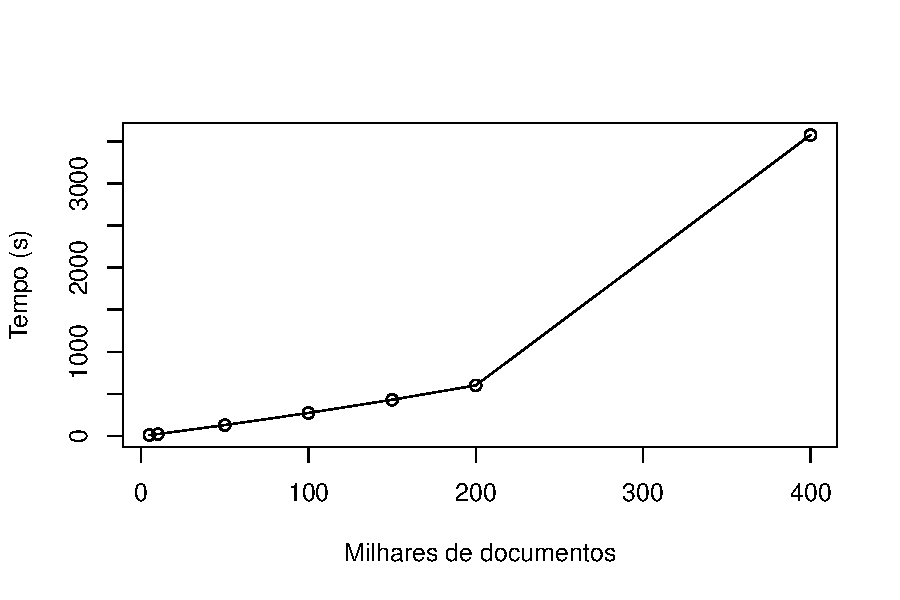
\includegraphics[width=.8\textwidth]{linechart.pdf}
\caption{Tempo de execução por tamanho da coleção}
\label{fig:time_vs_colsize}
\end{figure}


A tabela~\ref{tab:exec_time_buffer} mostra o tempo de execução total e de cada uma das três etapas para uma coleção de 50000 documentos, variando-se o tamanho do \emph{buffer}. É interessante notar que o tempo da etapa 2 tende a aumentar com um \emph{buffer} maior, mas em contrapartida o tempo da etapa 3 diminui. Isso intuitivamente faz sentido, pois quanto menor o buffer mais blocos existirão para se fazer o \emph{merge}.

O tempo total de indexação teve pouca variação, pelo \emph{tradeoff} entre as etapas 2 e 3. Uma observação a ser considerada é que o \emph{buffer} não é utilizado na primeira etapa, portanto o tamanho do mesmo não interfere no tempo desta etapa.

\begin{table}[ht]
\centering
\caption{Tempo de execução em segundos para \emph{buffer} de tamanho variado}
\label{tab:exec_time_buffer}
\begin{tabular}{rrrrr}
Buffer  & Etapa 1 & Etapa 2 & Etapa 3 & Total \\ \hline
2000    & 77      & 17      & 35      & 129 \\
4000    & 79      & 18      & 31      & 128 \\
8000    & 78      & 19      & 29      & 126 \\
16000   & 78      & 21      & 27      & 126 \\
32000   & 77      & 21      & 22      & 120 \\
64000   & 77      & 22      & 21      & 120 \\
128000  & 80      & 23      & 19      & 122 \\

\end{tabular}
\end{table}


\subsection{Espaço de armazenamento}

O tamanho do arquivo temporário necessário para a ordenação externa é função do número total de triplas escritas, sendo que cada uma delas ocupa o espaço de $3$ números inteiros de $4$ bytes. Por exemplo, o tamanho total sem compressão do arquivo temporário na execução de 50000 documentos foi de $138$ MB.

O índice invertido final contém dois arquivos. O primeiro é um lista de duplas $<documento, frequencia>$. O segundo armazena o vocabulário, contendo em cada entrada um apontador para o ínicio da lista invertida e o tamanho da mesma. Para os mesmos 50000 documentos exemplificados, o arquivo de listas ficou com $92$ MB e o arquivo de vocabulário com $31$ MB.


\section{Pendências e possíveis melhorias}

O salto na curva de execução descrito na seção~\ref{sec:time} ainda não está clara. Estou investigando o comportamento do sistema para entender o motivo da mesma.

Uma alternativa natural para obter melhor desempenho é o uso de compressão. Infelizmente não foi possível rodar experimentos usando compressão a tempo da escrita deste relatório, mas pretendo incorporar o uso da mesma no sistema, visando os próximos trabalhos.

Além disso, ainda não estão sendo tratadas da forma mais adequada as diferentes codificações de caracteres encontradas, resultando em problemas com caracteres acentuados em algumas situações.

%\bibliographystyle{sbc}
%\bibliography{tc}

\end{document}
